\documentclass[11pt]{amsart}
%%%%%%%%%%%%%% Packages
\usepackage{amssymb,amsfonts,amsthm,amsmath}
\usepackage[english]{babel}
\usepackage[all,cmtip]{xy}
\usepackage{tikz}
\usepackage{mathtools}
\usepackage{tensor}
\usepackage{csquotes}
\usepackage[vcentermath]{youngtab}
%\usepackage{stix}
\usetikzlibrary{arrows,chains,matrix,positioning,scopes}
%\usepackage{mathrsfs}
%\usepackage[notcite,notref]{showkeys}


%%%%%%%%%%% Tikz
\makeatletter
\tikzset{join/.code=\tikzset{after node path={%
\ifx\tikzchainprevious\pgfutil@empty\else(\tikzchainprevious)%
edge[every join]#1(\tikzchaincurrent)\fi}}}
\makeatother
\tikzset{>=stealth',every on chain/.append style={join},
         every join/.style={->}}

        

%%%%%%%%%%%% Personalized commands and environments

\newcommand{\inputc}[1]{ \raisebox{-0.5\height}{\input{#1}} }
\newtheorem{theorem}{Theorem}
\newtheorem{lemma}[theorem]{Lemma}
\newtheorem{corollary}[theorem]{Corollary}
\newtheorem{definition}[theorem]{Definition}
\newtheorem{proposition}[theorem]{Proposition}
\newtheorem{remark}[theorem]{Remark}
\newtheorem{example}{Example}
%\newtheorem{theorem*}{Theorem}

\newcommand{\func}[3]{{#1} : {#2} \longrightarrow {#3}}
\numberwithin{equation}{section}
\newcommand{\dbar}{\bar{\partial}}
\newenvironment{myproof}{\noindent{it Proof}
\setlength{\parindent}{0mm}}
{$\hfill \bs$}


%%%%%%%%%%%%%%%%%%%%%%%% Title and Author information

\title{MAT 303 Recitations: Week 12}


\author[M. Gomes]{Marlon de Oliveira Gomes}
\address{Mathematics Department 3-101, Stony Brook University,
100 Nicolls Road, Math Tower, 
Stony Brook, NY, 11794, USA} \email{mgomes@math.stonybrook.edu}



%%%%%%%%%%% Text
\begin{document}

\maketitle


\section*{Section 3.5: Nonhomogeneous Equations and Undetermined Coefficients}

We wrap up our discussion of section 3.5 with the method of Variation of Parameters. This is a strategy best suited to equations in which the usual method of Undetermined Coefficients fails (more on that below), but it works in general, at least in theory (in practice, some of the integrals involved may be far too complicated to be worth it, even for simple nonhomogeneous equations).

To make the exposition more concrete, we will stick to second-order equations, but the process can be applied to higher order equations by means of linear algebra. Our setup consists of a second-order differential equation with linear coefficients, 
\begin{equation}\label{model}
y''(t)+Py'(x)+Qy(x) = F(x),
\end{equation}
where $P,Q$ are constants. We've learned how to deal with such equations when $F(x)=0$, via the method of characteristics. We recall that a solution to the homogeneous counterpart of equation \eqref{model} is called a complementary solution. Here we assume this solution takes the form
\begin{equation*}
y_c(x)=C_1y_1(x)+C_2y_2(x),
\end{equation*}
where $y_1$ and $y_2$ are linearly independent, $C_1,C_2$ are constants (to be determined based upon initial conditions). The method of variation of parameters consists of a perturbation of the complementary solution
\begin{equation}\label{guess}
y(x)=u_1(x)y_1(x)+u_2(x)y_2(x),
\end{equation}
where $u_1, u_2$ are functions of $x$ to be determined. The goal is to replace the second-order equation on $y$ by a system of first-order equations on $u_1,u_2$, thus (conceptually) simplifying the problem.

As a first applicaiton of the method, we will use an example for which Undetermined Coefficients is more suitable than Variation of Parameters. The reader is invited to use the former as practice, and to verify the accuracy of our new method. 

\begin{example}
Consider the equation
\begin{equation*}
y^{''} + y = e^x.
\end{equation*}
The characteristic polynomial of its homogeneous counterpart is $p(r)=r^2+1$, with complex roots $\pm i$.  The complementary solution of the problem is 
\begin{equation*}
y_c(x)=A_1\cos(x)+A_2\sin(x).
\end{equation*}
We perturb it by setting 
\begin{equation*}
y(x)=u_1(x)\cos(x)+u_2(x)\sin(x),
\end{equation*}
for unknown functions $u_1,u_2$. The derivative of this guess is 
\begin{equation*}
y^{'}(x)=[u_{1}^{'}(x)\cos(x)+u_{2}^{'}(x)\sin(x)] -u_1(x)\sin(x)+u_2(x)\cos(x).
\end{equation*}
At this point we \underline{impose} a condition on the auxilliary functions $u_1,u_2$, to avoid the appearance of their second derivatives in subsequent steps, by setting the term in brackets to zero, 
\begin{equation}\label{example1_step1}
u_{1}^{'}(x)\cos(x)+u_{2}^{'}\sin(x)=0.
\end{equation}
We will continue our derivation of  $y$ and its derivatives under this assumption, that is, 
\begin{equation*}
y^{'}(x)= -u_1(x)\sin(x)+u_2(x)\cos(x),
\end{equation*}
so that 
\begin{equation*}
y^{''}(x) = -u_{x}^{'}(x)\sin(x)-u_1(x)\cos(x)+u_{2}^{'}(x)\cos(x)-u_2(x)\sin(x).
\end{equation*}
It follows that 
\begin{align}
\nonumber
y^{''}(x)+y(x) & =-u_{1}^{'}(x)\sin(x)+u_{2}^{'}(x)\cos(x) \\
\label{example1_step2}
e^{x} & = -u_{1}^{'}(x)\sin(x)+u_{2}^{'}(x)\cos(x) .
\end{align}
Combining equations $\eqref{example1_step1}$ and $\eqref{example1_step2}$, we obtain the desited system of linear, first-order equations on $u_1,u_2$:
\begin{align*}
u_{1}^{'}(x)\cos(x)+u_{2}^{'}(x)\sin(x) & =0\\
-u_{1}^{'}(x)\sin(x)+u_{2}^{'}(x)\cos(x) & = e^{x}.
\end{align*}
Here we note the importance of linear independence of the solutions to the homogeneous equation. For a fixed value of $x$, the system is solvable, since the determinant is their Wronskian:
\begin{equation*}
\det \left(
\begin{matrix}
\cos(x) & \sin(x) \\
-\sin(x) &  \cos(x) 
\end{matrix}
\right) = W(\cos(x), \sin(x)) = 1. 
\end{equation*}
We will solve the system by elimination. Multiplying the first equation by $\sin(x)$, the second by $\cos(x)$, and adding them, we obtain:
\begin{align*}
u_{2}^{'}(x) & = e^{x}\cos(x) \\
u_2(x) & = \int e^x\cos(x) dx \\
u_2(x) & =   \frac{e^{x}(\sin(x)+\cos(x))}{2}+ A_2.
\end{align*}
Using this we solve for $u_1$:
\begin{align*}
u_{1}^{'}(x)\cos(x)+u_{2}^{'}(x)\sin(x) & = 0 \\
u_{1}^{'}(x)\cos(x) + e^{x}\cos(x)\sin(x) & = 0\\
\cos(x)(u_{1}^{'}(x)+e^x\sin(x)) & =0.
\end{align*}
For this equality to hold everywhere, we must have 
\begin{align*}
u_{1}^{'}(x) & = -e^x\sin(x) \\
u_{1}(x) & = -\int e^{x}\sin(x)dx \\
u_{1}(x) & = \frac{e^{x}(\cos(x)-\sin(x))}{2} + A_1.
\end{align*}
We are now ready to write the general solution to the inhomogeneous problem:
\begin{align*}
y(x) & = u_1(x)\cos(x) + u_2(x)\sin(x) \\
& =\left[\frac{e^{x}(\cos(x)-\sin(x))}{2} + A_1\right]\cos(x) + \left[\frac{e^{x}(\cos(x)+\sin(x))}{2} + A_2\right]\sin(x)\\
& = \frac{e^x}{2}[\cos^2(x)-\sin(x)\cos(x)+\cos(x)\sin(x)+\sin^2(x)] + A_1\cos(x)+A_2\sin(x) \\
& = \frac{e^x}{2}+A_1\cos(x)+A_2\sin(x).
\end{align*}
\end{example}

The above example should serve as a cautionary tale: while variation of Parameters eliminates the guessing game from Undetermined Coefficients, it may lead to computations that are much longer than necessary.

Below are two other applications of this method that you can use as reference for problems 53 and 55. 

\begin{example}
The following example is extracted from problem 3.5.52. Consider the differential equation 
\begin{equation*}
y^{''}(x)+9y(x)=\sin(3x).
\end{equation*}
The complementary solutions take the form 
\begin{equation*}
y_c(x)=A_1\cos(3x)+A_2\sin(3x).
\end{equation*}
We learned last week that this is a case of duplication, and expect the particular solution to be of the form 
\begin{equation*}
y_p(x)=C_1x\cos(3x)+C_2x\sin(3x),
\end{equation*}
for certain constants $C_1,C_2$. Let's use variation of parameters to confirm our expectation. 

We begin with a perturbation of the complementary solution, 
\begin{equation*}
y(x)=u_{1}(x)\cos(3x)+u_2(x)\sin(3x),
\end{equation*}
whose derivative is 
\begin{equation*}
y^{'}(x)=[u_{1}^{'}(x)\cos(3x)+u_{2}^{'}\sin(3x)] -3u_1(x)\sin(3x)+3u_2(x)\cos(3x).
\end{equation*}
As before, we impose the condition that the term in brackets vanishes, 
\begin{equation}\label{example2_step1}
u_{1}^{'}(x)\cos(3x)+u_{2}^{'}\sin(3x) =0.
\end{equation}
We continue the derivation of $y$ with this assumption, 
\begin{equation*}
y^{'}(x)=-3u_1(x)\sin(3x)+3u_2(x)\cos(3x),
\end{equation*}
so,
\begin{equation*}
y^{''}(x) = -3u_{1}^{'}\sin(3x)+3u_{2}^{'}(x)\cos(3x) -9u_1(x)\cos(3x)-9u_2(x)\sin(3x),
\end{equation*}
hence 
\begin{align}
\nonumber
y^{''}(x)+9y(x) & = -3u_{1}^{'}\sin(3x)+3u_{2}^{'}(x)\cos(3x) \\
\label{example2_step2}
\sin(3x) & = -3u_{1}^{'}\sin(3x)+3u_{2}^{'}(x)\cos(3x).
\end{align}
We are now in possesion of the system of linear first-order equations for $u_1,u_2$: 
\begin{align*}
u_{1}^{'}(x)\cos(3x)+u_{2}^{'}(x)\sin(3x) & = 0, \\
-3u_{1}^{'}(x)\sin(3x)+3u_{2}^{'}\cos(3x) & = \sin(3x).
\end{align*}
These can be solved by elimination, resulting in 
\begin{align*}
u_{2}^{'}(x) & =  \frac{\cos(3x)\sin(3x)}{3} \\
u_{2}(x) & = \int \frac{\cos(3x)\sin(3x)}{3} dx \\
& = \int \frac{\sin(6x)}{6} dx \\
& = \frac{-\cos(6x)}{36} + C_2,
\end{align*}
and
\begin{align*}
u_{1}^{'}(x) & = -\frac{\sin^{2}(3x)}{3} \\
u_1(x) & =- \int \frac{\sin^{2}(3x)}{3}  dx \\
& = -\frac{1}{3}\int \frac{1-\cos(6x)}{2} dx\\
& = -\frac{x}{6} + \frac{\sin(6x)}{36} + C_1.
\end{align*}
We are now in a position to compute the solution, 
\begin{align*}
y(x) & = u_1(x)\cos(3x)+u_2(x)\cos(3x) \\
& = \left[-\frac{x}{6} + \frac{\sin(6x)}{36} + C_1 \right]\cos(3x) + \left[\frac{-\cos(6x)}{36} + C_2\right]\sin(3x) \\
& = -\frac{x\cos(6x)}{36} + \frac{\sin(6x)\cos(3x)}{36} + C_1\cos(3x) - \frac{\sin(3x)\cos(6x)}{36} + C_2\sin(3x) \\
& = C_1\cos(3x) + C_2\sin(3x) -\frac{x\cos(6x)}{36} +\frac{\sin(3x)}{36},
\end{align*}
where in the last equality we used the subtraction formula for the sine function. The last factor can be incorporated into the term $C_1\sin(3x)$, by changing the value of the constant, so we find the general solution
\begin{equation*}
y(x)= C_1\cos(3x) + C_2\sin(3x) -\frac{x\cos(6x)}{36}.
\end{equation*}
\end{example}

\begin{example}
In problem 3.5.54, we have a case in which Undetermined Coefficients doesn't work, the equation
\begin{equation*}
y^{''}(x)+y(x) = \csc^2(x).
\end{equation*}
As in example 1, the complementary solution is 
\begin{equation*}
y_c(x)=A_1\cos(x)+A_2\sin(x),
\end{equation*}
so we perturb it by setting 
\begin{equation*}
y(x)=u_1(x)\cos(x)+u_2(x)\sin(x).
\end{equation*}
Once more, we compute the derivative
\begin{equation*}
y^{'}(x)=[u_{1}^{'}(x)\cos(x)+u_{2}^{'}(x)\sin(x)] -u_1(x)\sin(x)+u_2(x)\cos(x),
\end{equation*}
and set the term in brackets to zero, 
\begin{equation}\label{example3_step1}
u_{1}^{'}(x)\cos(x)+u_{2}^{'}\sin(x)=0.
\end{equation}
Proceeding under this assumption, we compute the second derivative
\begin{equation*}
y^{''}(x) = -u_{x}^{'}(x)\sin(x)-u_1(x)\cos(x)+u_{2}^{'}(x)\cos(x)-u_2(x)\sin(x),
\end{equation*}
and input it into the differential equation to obtain
\begin{align}
\nonumber
y^{''}(x)+y(x) & =-u_{1}^{'}(x)\sin(x)+u_{2}^{'}(x)\cos(x) \\
\label{example3_step2}
\csc^2(x) & = -u_{1}^{'}(x)\sin(x)+u_{2}^{'}(x)\cos(x) .
\end{align}
We now have the system of equations in variables $u_1,u_2$:
\begin{align*}
u_{1}^{'}(x)\cos(x)+u_{2}^{'}(x)\sin(x) & =0\\
-u_{1}^{'}(x)\sin(x)+u_{2}^{'}(x)\cos(x) & = \csc^2(x).
\end{align*}
By elimination we find 
\begin{align*}
u_{2}^{'} & = \csc^2(x)\cos(x) \\
u_2(x) & = \int \csc^2(x)\cos(x) dx \\
& = -\csc(x)+A_2.
\end{align*}
Meanwhile, 
\begin{align*}
u_{1}^{'}(x) & = -\csc(x) \\
& = -\int \csc(x) dx \\
& = \log(\cot(x)+\csc(x))+A_1.
\end{align*}
Assembling these into the general solution, we have 
\begin{align*}
y(x) & = \left[\log(\cot(x)+\csc(x))+A_1\right]\cos(x) + \left[-\csc(x)+A_2\right]\sin(x)\\
& = A_1\cos(x) + A_2\sin(x) + \log(\cot(x)+\csc(x))\cos(x)-1.
\end{align*}
\end{example}

\section*{Section 3.6: Forced Oscillations}
In section 3.6 we bring the full power of the methods we learned throughout the chapter to bear on forced oscillations. The prototypical problem is a second-order differential equations with a simple harmonic inhomogeneous term, 
\begin{equation*}
mx^{''}(t)+cx^{'}(t)+kx(t) = F_0\cos(\omega t - \alpha).
\end{equation*}
We remark that by means of the relation $\sin(\omega t) = \cos\left(\omega t - \frac{\pi}{2}\right)$ we may also treat oscillations involving the sine function by this formalism. 

\begin{example}
In problem 3.6.2, we are given a differential equation
\begin{equation*}
x^{''}+4x=5\sin(3t),
\end{equation*}
with initial conditions $x(0)=0,x^{'}(0)=0$. Our goal is to find its solution, express it as a combination of two harmonic oscillations, one with natural frequency and one with external frequency, and plot the solution, identifying its period. 

The general complementary solution to the problem takes the form
\begin{equation*}
x_c(t)=A\cos(2t)+B\sin(2t)
\end{equation*}
whereas one expects a particular solutions to be written as 
\begin{equation*}
x_p(t)=C_1\sin(3t)+C_2\cos(3t).
\end{equation*}
Using the method of Undetermined Coefficients, we find the values $C_1=-1$ and $C_2=0$, thus we can write a solution to the inhomogeneous problem as 
\begin{equation*}
x(t)=A\cos(2t)+B\sin(2t) -\sin(3t).
\end{equation*}
The coefficients $A$ and $B$ are found by matching the initial data. We observe that 
\begin{equation*}
x^{'}(t)=-2A\sin(2t)+2B\cos(2t)-3\cos(3t),
\end{equation*}
so that the conditions at $t=0$ amount to 
\begin{align*}
 A  & = 0 \\ 
 2B-3 & = 0,
\end{align*}
which gives
\begin{equation*}
x(t)=\frac{3}{2}\sin(2t)-\sin(3t),
\end{equation*}
a periodic function with period $2\pi$. Below is a plot of its graph, the marked points corresponding to periods.
\begin{center}
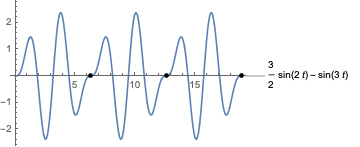
\includegraphics[width=0.8\textwidth]{p3.png} 
\end{center}
\end{example}

Below is a variation of problems 3.5.11 and 3.5.12, in which we are meant to find the steady periodic solution and the actual solution corresponding to given intial data.
\begin{example}
Consider the equation
\begin{equation*}
x^{''}(t)+2x^{'}(t)+2x(t) = 3\cos(2t),
\end{equation*}
with initial conditions $x(0)=0$, $x^{'}(0)=0$. The characteristic polynomial of this equation is 
\begin{equation*}
r^2+2r+2=(r+1)^2+1,
\end{equation*}
with roots $-1\pm i$. Complementary solutions take the form
\begin{equation*}
x_{c}(t)=Ce^{-t}\cos(t-\alpha),
\end{equation*}
for constants $C$ and $\alpha$ to be determined, whereas we expect a particular solution to be of the form 
\begin{equation*}
x_p(t)=A\cos(2t)+B\sin(2t).
\end{equation*}
Its derivatives are 
\begin{align*}
x_{p}^{'}(t) & = -2A\sin(2t)+2B\cos(2t), \\
x_{p}^{''}(t) & = -4A\cos(2t)-4B\sin(2t).
\end{align*}
Combining the derivatives according to the equation, we obtain 
\begin{align*}
x_{p}^{''}(t)+2x_{p}^{'}(t)+2x_p(t) & =  3\cos(2t) \\
(-2A+4B)\cos(2t)+(-2B-4A)\sin(2t) & =  3\cos(2t),
\end{align*}
so we find $A=-\frac{3}{10}$, and $B=\frac{3}{5}$. 

An actual solution to the problem takes the form
\begin{equation*}
x(t)=Ce^{-t}\cos(t-\alpha)-\frac{3}{10}\cos(2t)+\frac{3}{5}\sin(2t),
\end{equation*}
with derivative
\begin{equation*}
x'(t)=-Ce^{-t}[\cos(t-\alpha)+\sin(t-\alpha)]+\frac{3}{5}\sin(2t)+\frac{6}{5}\cos(2t).
\end{equation*}
Taking into account initial conditions, we have 
\begin{align*}
C\cos(\alpha) - \frac{3}{10} & = 0 \\
-C\cos(\alpha)+C\sin(\alpha)+\frac{6}{5} & = 0,
\end{align*}
whose solutions are $C=\frac{3\sqrt{10}}{10}$, $\alpha =2\pi-\arctan(3) \approx 5.03$. 

The final form of the solution is 
\begin{equation*}
x(t)=\frac{3\sqrt{10}}{10}e^{-t}\cos(t-\arctan(3)) -\frac{3}{10}\cos(2t)+\frac{3}{5}\sin(2t),
\end{equation*}
and the corresponding steady periodic solution is 
\begin{equation*}
x_{sp}(t) =  -\frac{3}{10}\cos(2t)+\frac{3}{5}\sin(2t) = \frac{3\sqrt{5}}{10}\cos(2t-\arctan{2}).
\end{equation*}
\end{example}
\begin{thebibliography}{0}

\bibitem{EdPeCa} C. Henry Edwards, David E. Penney and David T. Calvis, {\it Differential Equations and Boundary Value Problems: Computing and Modelling}, 5th edition, Pearson, 2014.

\end{thebibliography}
\end{document}


